\section{Subagents, cascades and the moves of a proof}\label{sec:agents}

A working BLLM is not one generator and one check. A coordinator hands parts of a problem to subagents, each subagent proposes candidates by its own method, and the candidates meet checks of very different cost: a test that runs in a millisecond, a randomized identity test, a full proof checker. This section proves the two laws that govern such a system. Splitting the work among subagents costs nothing, provided each receives a share of the budget proportional to its total cost, and a misallocated budget is charged exactly a Kullback--Leibler divergence (Theorem~\ref{thm:H}). Cheap unreliable checks placed before an exact one make the exact check paid, up to a logarithmic premium, only on the correct candidates (Theorem~\ref{thm:cascade}). The section ends with the six moves by which the subagents of Section~\ref{sec:cases} propose candidates.

\subsection{Subagents}

Partition the candidates into groups $G_{1},\dots,G_{m}$, one for each subagent. Write $A_{k}=\sum_{i\in G_{k}}a_{i}$, $P_{k}=A_{k}/A$ for the share of the $k$-th subagent and $p^{(k)}=(a_{i}/A_{k})_{i\in G_{k}}$ for its own cost profile. A coordinator gives the $k$-th subagent a budget $\theta_{k}>0$ with $\Theta=\sum_{k}\theta_{k}\le\theta$, and the subagent schedules its checks with any $\theta_{k}$-sound schedule. The union of the schedules is $\theta$-sound, since the expected numbers of false acceptances add.

\begin{mainthm}[Subagents]\label{thm:H}
\begin{enumerate}[label=\textup{(\roman*)},leftmargin=2.2em,itemsep=1pt]
\item \emph{Chain rule.} $H(p)=H(P)+\sum_{k}P_{k}H(p^{(k)})$.
\item \emph{Price of a split.} The sum over the subagents of the lower bounds of Theorem~\ref{thm:A} for their groups exceeds the lower bound for the whole profile by exactly
\begin{equation}\label{eq:splitprice}
\frac{A}{L}\Bigl(D(P\,\|\,q)+\log\frac{\theta}{\Theta}\Bigr),\qquad q_{k}=\frac{\theta_{k}}{\Theta},
\end{equation}
where $D$ is the Kullback--Leibler divergence. It vanishes if and only if $\theta_{k}=\theta P_{k}$ for every $k$.
\item \emph{Coordination by one number.} If $\theta_{k}=\theta P_{k}$, the optimal schedule of Theorem~\ref{thm:A} computed by the $k$-th subagent from its own costs and the single number $\theta P_{k}$ coincides on $G_{k}$ with the optimal schedule of the whole profile. The union is $\theta$-sound and costs at most $\frac AL(H(p)+\log\frac1\theta)+A$.
\item \emph{Hierarchies.} For a tree of subagents in which every node passes to each child the share of its own budget proportional to the child's total cost, the schedule at the leaves is the optimal flat schedule, and
\begin{equation}\label{eq:treeentropy}
A\,H(p)=\sum_{v}A_{v}\,H(P^{v}),
\end{equation}
the sum over the internal nodes $v$ of the tree, where $A_{v}$ is the total cost below $v$ and $P^{v}$ the distribution of $A_{v}$ among the children of $v$.
\end{enumerate}
\end{mainthm}

\begin{proof}
(i) For $i\in G_{k}$, $\log(A/a_{i})=\log(A/A_{k})+\log(A_{k}/a_{i})$; multiply by $a_{i}$, sum over $i\in G_{k}$ and then over $k$, and divide by $A$.

(ii) The lower bounds for the groups add up to $\frac1L\sum_{k}\bigl(A_{k}H(p^{(k)})+A_{k}\log\frac1{\theta_{k}}\bigr)$. By (i), subtracting $\frac AL(H(p)+\log\frac1\theta)$ leaves
\[
\frac1L\Bigl(\sum_{k}A_{k}\log\frac1{\theta_{k}}-A\,H(P)-A\log\frac1\theta\Bigr)=\frac AL\sum_{k}P_{k}\log\frac{\theta P_{k}}{\theta_{k}}=\frac AL\Bigl(\sum_{k}P_{k}\log\frac{P_{k}}{q_{k}}+\log\frac\theta\Theta\Bigr).
\]
Both terms are nonnegative, the first by Gibbs' inequality (Lemma~\ref{lem:gibbs}), and they vanish together exactly when $q=P$ and $\Theta=\theta$, that is, when $\theta_{k}=\theta P_{k}$.

(iii) The ceiling schedule of the $k$-th group at budget $\theta P_{k}$ gives $i\in G_{k}$ the number of runs $\lceil\frac1L\log\frac{A_{k}}{\theta P_{k}a_{i}}\rceil=\lceil\frac1L\log\frac{A}{\theta a_{i}}\rceil$, which is the flat ceiling schedule; its soundness and cost are those of Theorem~\ref{thm:A}.

(iv) By induction on the depth, applying (iii) at the root and the induction hypothesis to each subtree with its proportional budget. The identity \eqref{eq:treeentropy} follows by applying (i) at every internal node.
\end{proof}

The theorem has a practical reading. A coordinator need not know the costs of the individual checks of its subagents, and a subagent need not know anything about the others: one number per subagent, its share $\theta P_{k}$ of the budget, is enough to reach the global optimum, and the identity \eqref{eq:treeentropy} says that the entropy tax is paid node by node along the tree of delegation, each node paying for the uncertainty of its own split. A coordinator that splits the budget evenly among $m$ subagents instead pays the extra $\frac AL D(P\,\|\,u)=\frac AL(\log m-H(P))$, where $u$ is uniform, and this is unbounded when a few subagents carry almost all the cost.

\subsection{Weak checks before strong ones}

Let a fraction $\rho\in(0,1)$ of the candidates be incorrect. A \emph{strong check} costs $c$ and is exact: it accepts the correct candidates and rejects the others, as a proof checker does on a formal proof. A \emph{weak check} costs $b$ per run, has perfect completeness and soundness $\eps$: a language model asked to find a flaw, a numerical test at random points, a type check. A \emph{cascade} with $r$ weak runs runs the weak check $r$ times on every candidate and the strong check on the candidates that pass them. It keeps exactly the correct candidates, whatever $r$, so its soundness is that of the strong check alone.

\begin{theorem}[Weak before strong]\label{thm:cascade}
If the weak check attains its soundness, the expected cost of a cascade with $r$ weak runs per candidate is
\[
E(r)=br+c(1-\rho)+c\rho\,\eps^{r},
\]
and for $b\le c\rho L$,
\begin{equation}\label{eq:cascade}
c(1-\rho)+\frac bL\Bigl(1+\log\frac{c\rho L}{b}\Bigr)\ \le\ \min_{r\in\NN}E(r)\ \le\ c(1-\rho)+\frac bL\Bigl(1+\log\frac{c\rho L}{b}\Bigr)+b,
\end{equation}
the upper bound being attained up to $b$ by $r=\lceil\frac1L\log\frac{c\rho L}{b}\rceil$. Without weak checks the cost is $c$.
\end{theorem}

\begin{proof}
A correct candidate passes the $r$ weak runs and reaches the strong check; an incorrect one reaches it with probability $\eps^{r}$. This gives $E(r)$. Put $y=c\rho\eps^{r}$, so that $r=\frac1L\log\frac{c\rho}{y}$ and
\[
br+c\rho\eps^{r}-\frac bL\Bigl(1+\log\frac{c\rho L}{b}\Bigr)=\frac bL\Bigl(\frac{yL}{b}-1-\log\frac{yL}{b}\Bigr)\ge0
\]
by $\log x\le x-1$. This is the lower bound. For the upper bound let $x=\frac1L\log\frac{c\rho L}{b}\ge0$ and $r=\lceil x\rceil$. Then $br\le bx+b$ and $\eps^{r}\le\eps^{x}=b/(c\rho L)$, so $c\rho\eps^{r}\le b/L$.
\end{proof}

The strong check is thus paid on a fraction $1-\rho$ of the candidates, the correct ones, plus a premium logarithmic in $c/b$. When most proposals are wrong, as for a language model that guesses the next step of a hard proof, the saving is close to the factor $1/(1-\rho)$. With a proof checker of cost $c=1000$, a weak check of cost $b=1$ and soundness $\frac12$, and nine proposals in ten wrong, the best cascade runs nine weak checks per candidate and costs $110.8$ against $1000$; the lower bound is $110.7$.

The proof shows something more important than the saving. The soundness of the cascade does not depend on $\eps$: a weak check, however unreliable, can only remove candidates, never admit one. A learned critic may therefore be used freely as a filter, and only as a filter; the decision belongs to the exact check. The same holds with a randomized strong check of soundness $\eps_{s}$ given $r_{s}$ runs, whose false acceptances are bounded by $\rho\eps^{r}\eps_{s}^{r_{s}}\le\rho\eps_{s}^{r_{s}}$, so the weak runs may also be counted towards the budget of Theorem~\ref{thm:A} but are never needed for it.

\subsection{The moves of a proof}\label{ssec:moves}

The formal proofs of Section~\ref{sec:cases} are built from a small number of moves, used over and over. We name six, and the BLLM package of Section~\ref{sec:cases} has one subagent for each. A move is a way of generating candidates; it carries no authority of its own, and every candidate it produces meets the same checks, so Theorems~\ref{thm:A} to~\ref{thm:H} and~\ref{thm:cascade} apply to any mixture of moves.

\emph{Construction} produces an explicit object, a flow, a lattice, a cycle, a schedule, together with the statement that it has the required property, which is then checked. \emph{Strong then weak} proposes the strongest statement first and, when it is rejected, the next rung of a ladder of weakenings: a special case, a bounded range, a conditional form. Each rung is a candidate and enters the cost profile of Theorem~\ref{thm:A}. \emph{Residual} turns a partial success into a new goal, the part that remains unproved; it is the retry of Theorem~\ref{thm:B}, and when the corrections go on without end, as in a construction corrected to every order, whether the infinite sequence can be certified at finite cost is decided by Theorem~\ref{thm:E} and, without knowledge of the future corrections, by Corollary~\ref{cor:onlinesing}. \emph{Trivialization} specialises the parameters of a goal until it becomes a finite computation, which a kernel decides exactly, so that its check has soundness zero. \emph{Bypass} replaces a step by a result already kept in memory, whose check has been paid once. \emph{Blow-up} searches for a singular object or a counterexample.

\begin{remark}[Refutations carry no entropy tax]\label{rem:refutation}
A counterexample checked by exact evaluation needs one run, whatever the budget, because its check has soundness zero; so do the finite computations produced by trivialization and the results reused by bypass. In a mixed profile the entropy of Theorem~\ref{thm:A} is therefore the entropy of the candidates whose checks are randomized, with total cost $A_{\mathrm{rand}}$, and the exact checks add their cost once. A system that turns more of its work into exact checks lowers both $A_{\mathrm{rand}}$ and the entropy it pays on it.
\end{remark}

Figure~\ref{fig:agents} shows the arrangement: a coordinator, six subagents, a cascade of weak and strong checks, and a memory that stores every kept result as a note linked to the results it uses.

\begin{figure*}[t]
\centering
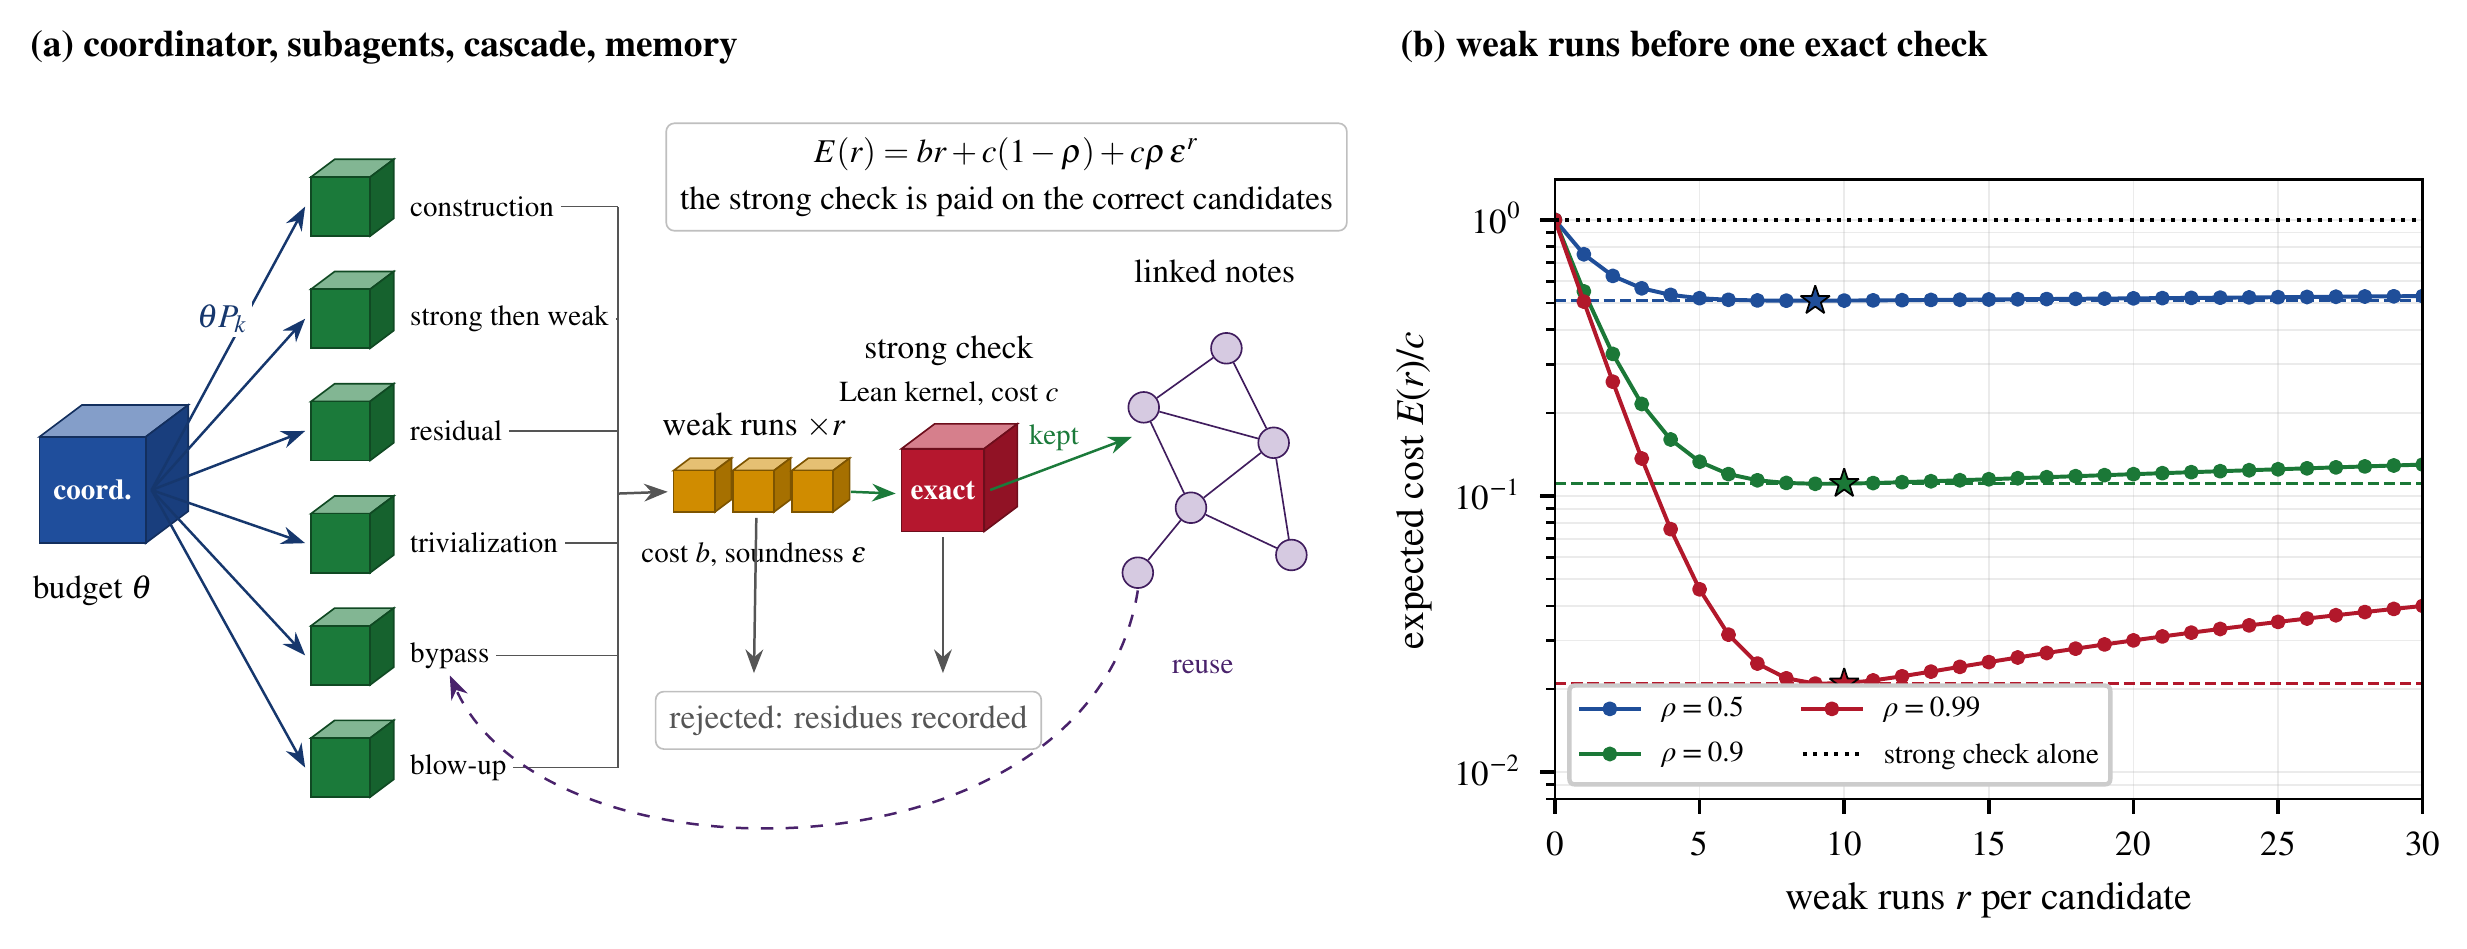
\includegraphics[width=0.98\textwidth]{figures/fig_agents}
\caption{Subagents and cascades. (a) A coordinator passes to each of six subagents, one for each move of Section~\ref{ssec:moves}, the share $\theta P_{k}$ of the budget proportional to its total cost (Theorem~\ref{thm:H}); every candidate meets a cascade of $r$ weak runs and one exact strong check (Theorem~\ref{thm:cascade}), and the kept results are stored as linked notes that the bypass move reuses. (b) The expected cost $E(r)/c$ of a cascade against the number $r$ of weak runs, for $b/c=10^{-3}$, $\eps=\frac12$ and $\rho\in\{0.5,0.9,0.99\}$; stars mark the number of runs of Theorem~\ref{thm:cascade}, the lower bound of \eqref{eq:cascade} is dashed and the cost $1$ of the strong check alone dotted.}
\label{fig:agents}
\end{figure*}
